\documentclass[11pt]{article}
\usepackage{times}
\usepackage{amsmath,amsthm,amssymb,mathtools,setspace,enumitem,epsfig,titlesec,verbatim,color,array,multirow,comment,graphicx,hyperref,blkarray}
%\usepackage[sort&compress]{natbib} % ProcB
\usepackage[super,sort&compress,comma]{natbib} % NComms
\usepackage[bf,small]{caption}
\usepackage[export]{adjustbox}
\usepackage[top=2.5cm,left=2.8cm,right=2.8cm,bottom=3.2cm]{geometry} 
\smallskip 

\definecolor{darkred}{rgb}{0.6,0,0}
\definecolor{darkblue}{rgb}{0,0.3,0.8}

\newcommand{\christian}[1]{\textcolor{blue}{{\bf CH:} #1}} 

\titleformat{\section}{\sffamily \fontsize{12}{20}\bfseries}{\thesection}{1em}{}
\titleformat{\subsection}{\sffamily \fontsize{11}{20}\bfseries}{\thesubsection}{1em}{}

\renewcommand{\figurename}{Supplementary Figure}


\newcommand{\FigIllustration}{{\bf Fig.~1}}

\newtheoremstyle{plainCl1}% name
{9pt}%      Space above, empty = 'usual value'
{15pt}%      Space below
{\it}% 	   Body font
{}%         Indent amount (empty = no indent, \parindent = para indent)
{\bfseries}% Thm head font
{.}%        Punctuation after thm head
{2mm}% Space after thm head: \newline = linebreak
{}%         Thm head spec

\newtheoremstyle{plainCl2}% name
{9pt}%      Space above, empty = 'usual value'
{15pt}%      Space below
{\it}% 	   Body font
{}%         Indent amount (empty = no indent, \parindent = para indent)
{\bfseries}% Thm head font
{.}%        Punctuation after thm head
{4mm}% Space after thm head: \newline = linebreak
{}%         Thm head spec

\theoremstyle{plainCl1}
\newtheorem{theorem}{Theorem}
\newtheorem{Prop}{Proposition}
\newtheorem{definition}{Definition}

\theoremstyle{plainCl2}
\newtheorem{lemma}{Lemma}
\newtheorem{proposition}{Proposition}
\newtheorem{Corollary}{Corollary}


\newcommand{\ALLD}{\emph{D}}

\newcommand{\A}{\mathbf{A}}
\newcommand{\abf}{\mathbf{a}}
\newcommand{\T}{\mathbf{T}}
\newcommand{\ubf}{\mathbf{u}}
\newcommand{\C}{\mathrm{C}}
\newcommand{\D}{\mathrm{D}}

\title{\sffamily \Large Supplementary Information\\[0.1cm] {\bfseries Introspection dynamics in asymmetric multiplayers games}}
\date{\empty}
\author{\parbox[c]{16cm}{\centering \onehalfspacing \fontsize{11}{12}\selectfont Marta Couto$^1$ and Saptarshi Pal$^1$\\[0.2cm]
$^1$Max Planck Research Group Dynamics of Social Behavior, Max Planck Institute for Evolutionary Biology, 24306~Ploen, Germany}}


\begin{document}
\maketitle
\onehalfspacing
\section*{Supplementary Figures: Asymmetric general public goods game}



\begin{figure}[h!]
\centering
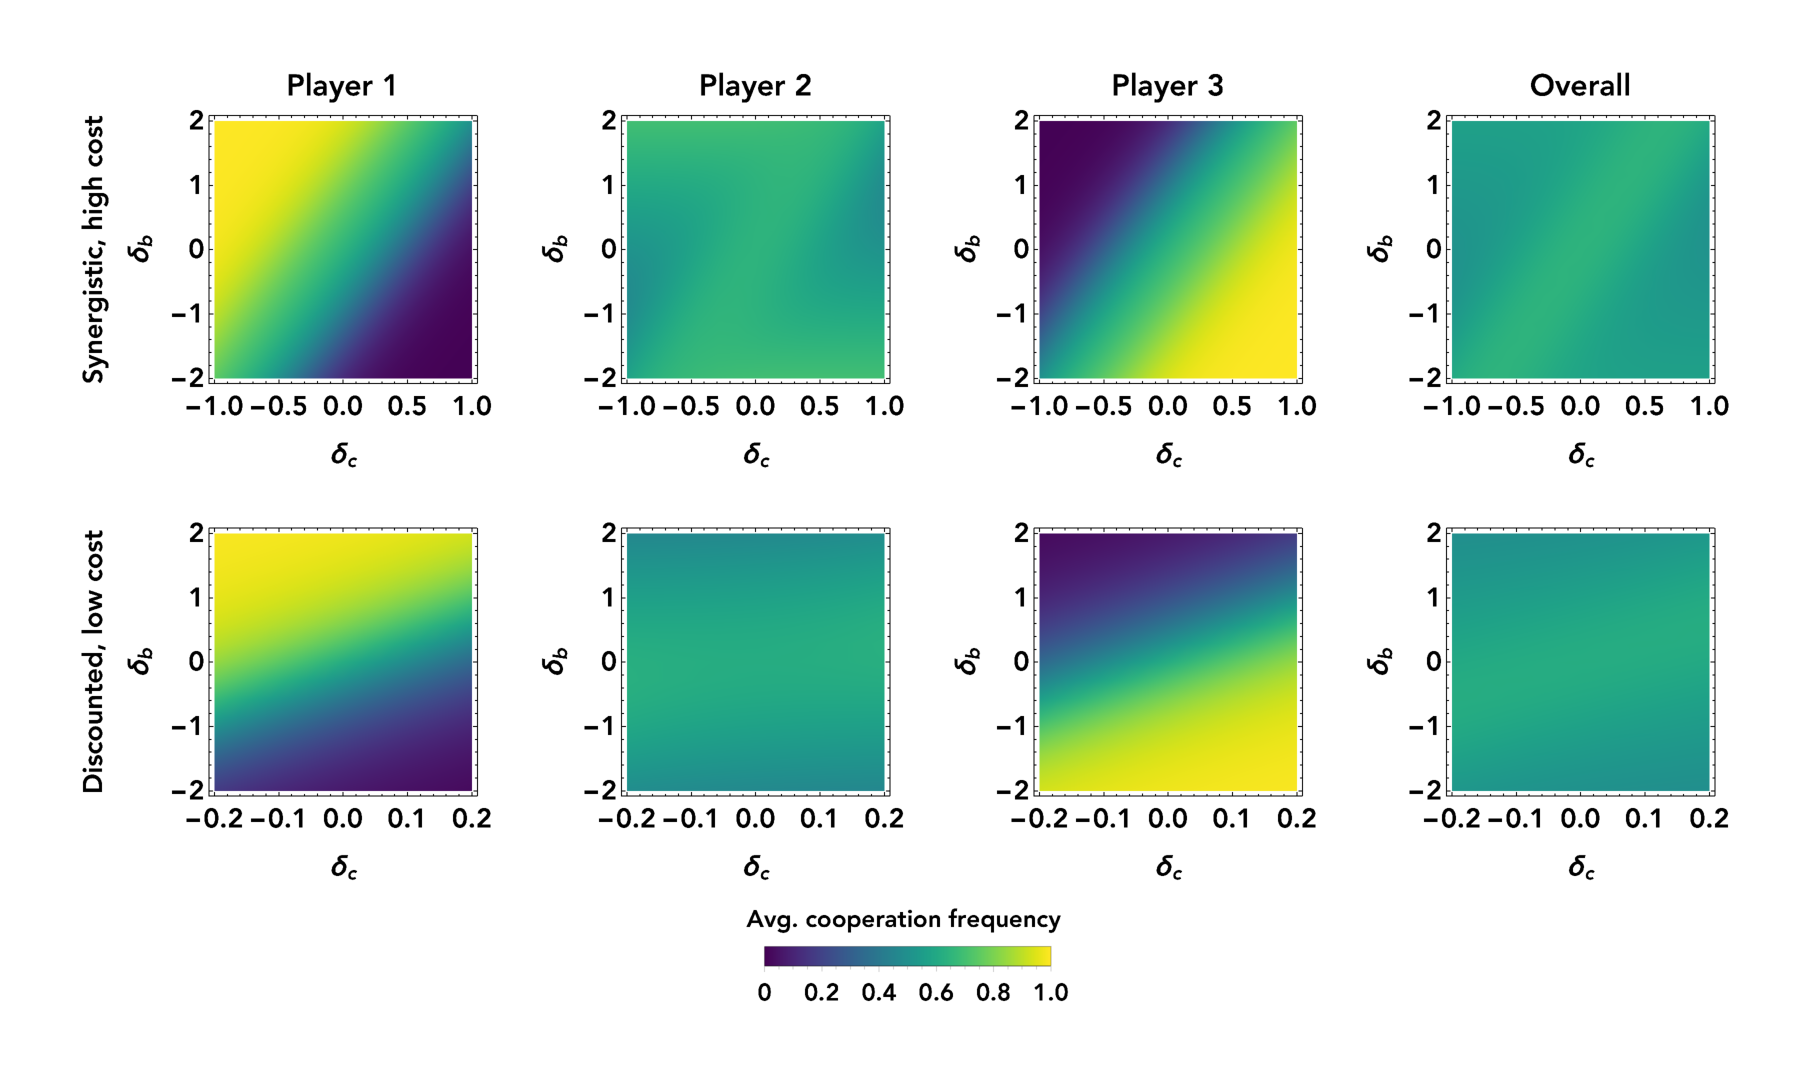
\includegraphics[width =  \textwidth]{figures/Supfigure1.eps}~\\[0.4cm]
\caption{\onehalfspacing
\textbf{Introspection dynamics in general public goods game with asymmetric players. We show stationary properties of the dynamics in a game with particular values of synergy/discount parameter and reference cost.} For a detailed description of the game, please see the section on general public goods game the main text. The setup is the same as Figure 3 of main text. There are three players with asymmetric costs and benefits. The respective costs for player 1, 2 and 3 are $c + \delta_c, c$, and $c - \delta_c$ respectively. The respective benefits they provide upon cooperation are $b + \delta_b, b$ and $b - \delta_b$ respectively. The parameters $c$ and $b$ respectively are the cost and benefits of the reference player (player 2). In here, we look at the cooperation probability for each player (and also overall cooperation) in stationary distribution of the introspection process. Players use a selection strength of $\beta = 5$. In the top row, we i) set the public good to be synergistic $w = 1.5$ and ii) allow a high reference cost, $c = 1$. In the bottom row, we i) set the public good to be discounted $w = 0.5$ and ii) allow a low reference cost $c = 0.2$. }
 
\label{Fig:Supp-Fig1}
\end{figure}
\clearpage

\begin{figure}
\centering
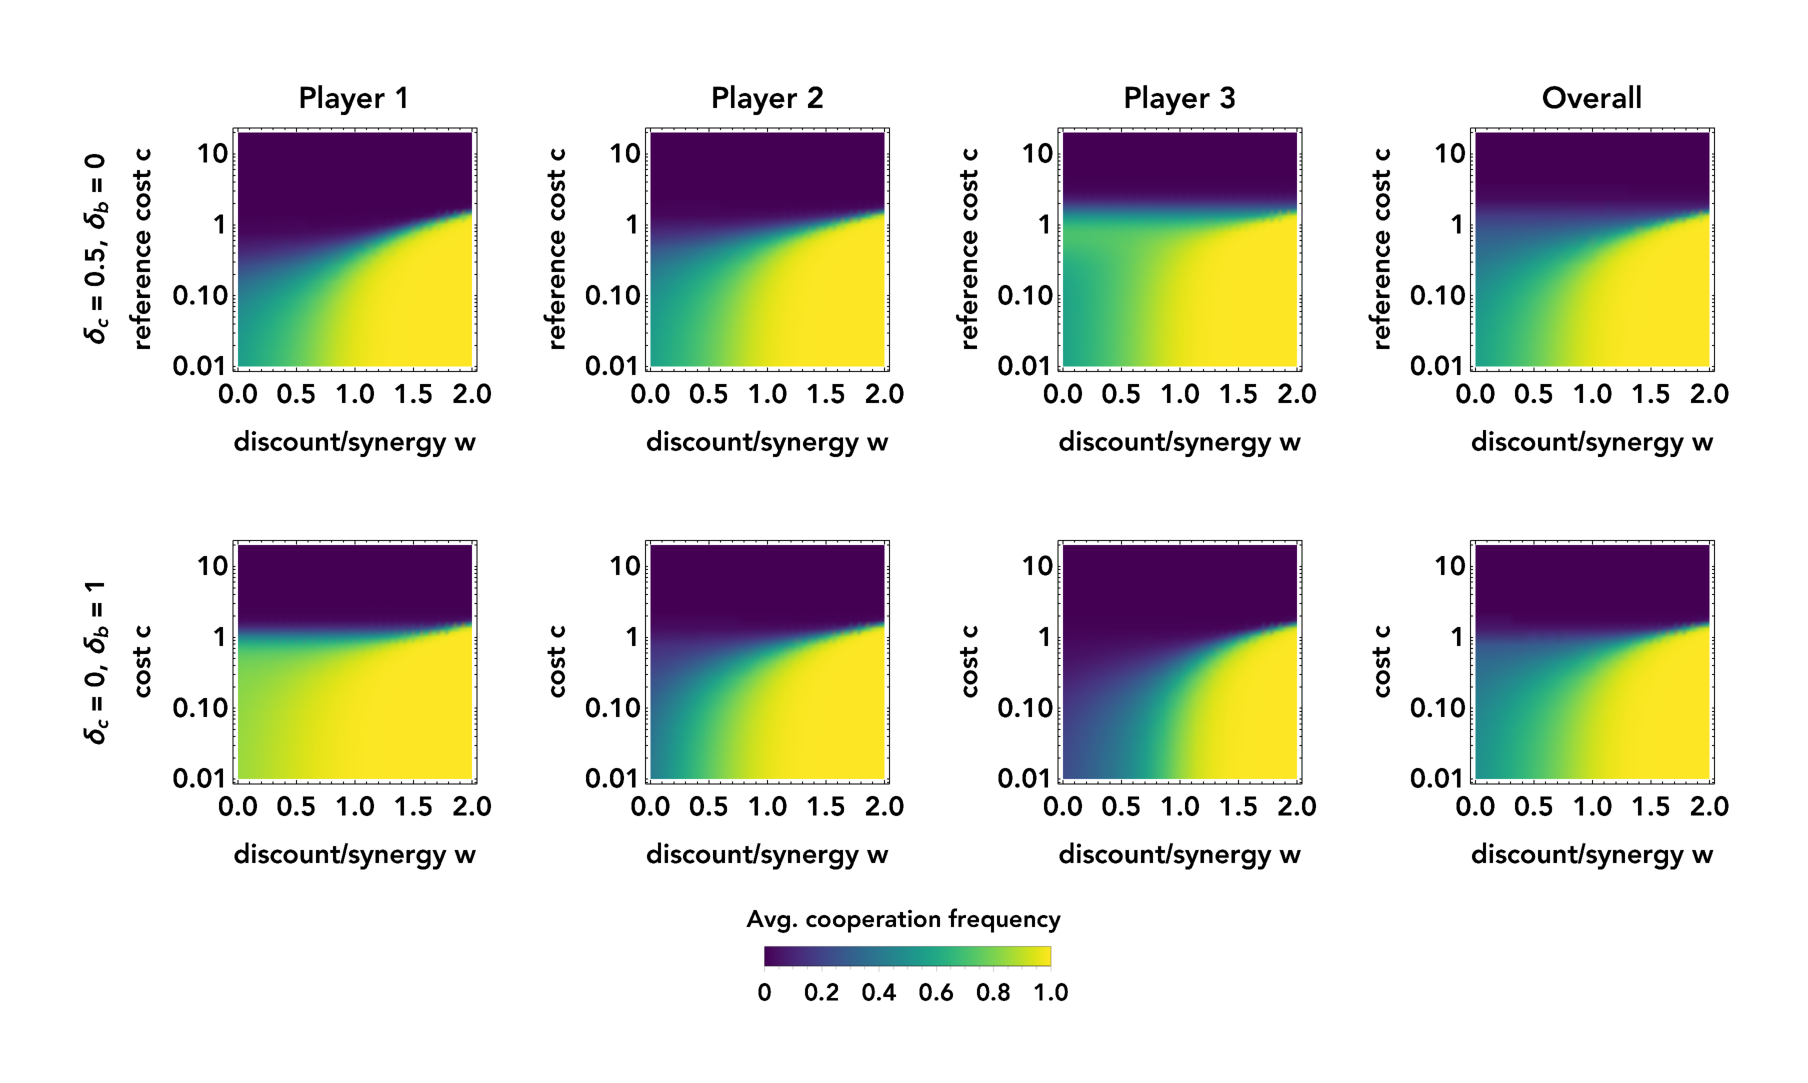
\includegraphics[width =  \textwidth]{figures/Supfigure2.eps}~\\[0.4cm]
\caption{\onehalfspacing
\textbf{Introspection dynamics in general public goods game with asymmetric players. We show stationary properties of the dynamics in a game with fixed asymmetry strengths.} For a detailed description of the game, please see the section on general public goods game in the main text. The setup is the same as Supplementary Figure \ref{Fig:Supp-Fig1}. In here, we show the cooperation probability of each player (and also the overall cooperation) in the stationary distribution of the introspection process versus the reference cost $c$ (cost of player 2) and tthe synergy/discount factor of the public good, $w$. For each row, the strength of asymmetry between the players is fixed. In the top row, the players do not differ in their benefits (they all have a benefit of value 2) but player 1 and player 3 have their cost of cooperation 0.5 units higher and lower respectively than player 2 (cost of cooperation for player 2 is varied in the y-axis). In the bottom row, all the players have the same cost of cooperation, $c$ (which is varied in the y-axis). In this case, player 1, 2 and 3 generate asymmetric benefits. Player 1,2 and 3 generate, 3, 2 and 1 units of benefits. 
}
\label{Fig:Supp-Fig2}
\end{figure}
\end{document}